\documentclass{standalone}
\usepackage{tikz,ctex}
\usepackage{tikz-3dplot} % 2-1
\usepackage{unicode-math} % 2-5,4-1,4-2
\setmathfont{Fira Math Regular}
\setmainfont{Fira Sans}
\definecolor{background}{RGB}{239, 239, 239} % 4-5,6-2,6-5
\begin{document}
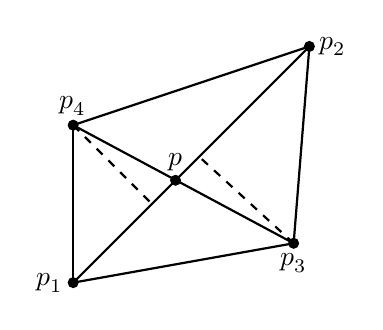
\begin{tikzpicture}
\def \p#1#2#3#4#5{\fill (#2,#3) circle(2pt) coordinate(#1) node[#5]{$#4$};}
\p{1}{0}{0}{p_1}{left}
\p{2}{3}{3}{p_2}{right}
\p{3}{2.8}{.5}{p_3}{below}
\p{4}{0}{2}{p_4}{above}
\p{5}{1.3}{1.3}{p}{above}
\foreach \u in{1,...,4}
\foreach \v in{\u,...,4}
    \draw[thick] (\u)--(\v);
\draw[dashed,thick] (4)--(1,1);
\draw[dashed,thick] (3)--(1.6,1.6);
\end{tikzpicture} 
\end{document}